\clearpage
\vspace*{\stretch{2}}%{\fill}
\begin{center}
\begin{minipage}{.75\textwidth}
\section{Sensado colaborativo para servicios telemáticos}

El sensado colaborativo es una técnica que permite obtener datos sensados de una ubicación física utilizando la colaboración de un número indeterminado de dispositivos provistos de sensores. Utilizando esta técnica de sensado se puede favorecer el acceso a servicios telemáticos sin intercambio económico. En este capítulo presentamos las ideas básicas del sensado colaborativo y su aplicación para el acceso gratuito a Internet a través de una red WiFi con infraestructura de una sola celda. % \pagebreak
\end{minipage}
\end{center}
\vspace{\stretch{3}} % \vfill % equivalent to \vspace{\fill}
\clearpage% https://tex.stackexchange.com/questions/70714/center-horizontally-and-vertically-a-block-of-text
\subsection{Introducción}

Hoy en día existe una gran cantidad de dispositivos de sensado de propiedades físicas haciendo posible la implantación del paradigma IoT. En este paradigma se aprovecha la cantidad masiva de sensores desplegados a lo largo y ancho de todo el mundo para obtener mediciones de parámetros físicos de interés. Además, estos datos se pueden transportar a lo largo y ancho de todo el mundo a través de Internet. Nosotros no estamos interesados en sensores insertados en un dispositivo electrónico miniaturizado empotrados y funcionando de forma autónoma. Estamos interesados en aquellos sensores que se implantan como parte de otros dispositivos, como pueden ser los relojes sofisticados (\emph{smartwatches}), los teléfonos móviles sofisticados (\emph{smartphones}), las tabletas portables o los computadores portátiles de media-alta gama.

Los dispositivos anteriores son capaces de incluir sensores (en un sentido amplio del significado de sensado) de: temperatura, acelerómetro (que permite averiguar datos sobre el movimiento de personas), nivel de señal electromagnética para comunicación inalámbrica (un ejemplo es el \emph{Received Signal Strength Indicator} (\acrshort{RSSI})), las imágenes (mediante una o varias cámaras fotográficas), de ruido o sonido ambiente (mediante un micrófono) o imágenes y sonido o ruido en movimiento (vídeo)...

Un detalle muy importante es que una gran parte de los ciudadanos actualmente disponen de alguno de los dispositivos anteriores. Además, siempre los llevan consigo a todos sus quehaceres diarios y cada vez se utilizan para hacer muchos de estos quehaceres cotidianos. Esto significa que cada persona que deambule por una ciudad diariamente es susceptible de recoger una gran cantidad de datos sensados del entorno que le rodea, sin hacer ningún esfuerzo adicional. Un ejemplo usual es el de un ciudadano que camina diariamente desde su casa hasta la sede de su trabajo llevando consigo su teléfono móvil sofisticado. Bastaría que diera una sola vez los permisos adecuados, para que su teléfono móvil se encargara de contar el número de pasos que ha dado, distribuirlos por metros recorridos y tiempo que ha tardado en darlos. Si además se ha medido el nivel de oxígeno en la sangre, a través del sensor adecuado del teléfono móvil, al comienzo y al final del recorrido, y tiene el software adecuado, se le puede avisar del nivel de stress que ha sufrido en su esfuerzo e incluso recomendándole que camine de otra forma diferente. Este no es más que un ejemplo sencillo de cómo utilizar \emph{individualmente} los sensores de un dispositivo móvil. Nosotros estamos interesados en el uso de estos sensores para realizar tareas colaborativas.

\subsection{Introducción al sensado colaborativo mediante teléfonos móviles}

La técnica de sensado móvil (\emph{mobile sensing}) \cite{MobileSensing} es aquella que en sentido amplio permite usar el teléfono móvil para sensar datos del entorno compartiéndolos con otros entes (personas o máquinas), para lograr llevar a cabo una tarea en común.

Ejemplos de sistemas en los que se puede emplear esta técnica es un sistema de aparcamiento colaborativo. Supongamos que una persona acude a un gran aparcamiento de un gran centro comercial, con la cámara fotográfica del teléfono móvil es capaz de captar imágenes de aparcamientos que están vacíos y su identificación. Acto seguido, una aplicación identifica al aparcamiento vacío y automáticamente envía su identificación de a un servidor en la Nube, junto con una etiqueta de tiempo que indica el momento del día en que fue recogida dicha información. Un procesado en la Nube de todas las identificaciones que se reciben puede exportar (para accederlos mediante una aplicación móvil), un listado de aparcamientos libres en un momento dado. Entonces, un usuario que desee aparcar en dicho aparcamiento, antes de acudir hasta él, o cuando está en el camino para acudir a él, podría consultar dicha información y hacer una estimación de cuándo podría llegar al aparcamiento. Si además recibe información del Centro comercial indicando cuántos coches hay cerca de esos aparcamientos libres, cuántos están entrando al aparcamiento y cuantos están saliendo, entonces, el conductor se podría hacer una idea de si le vale la pena intentar acudir a un aparcamiento concreto o bien dirigirse a otro. En este ejemplo, el principal objetivo es compartir información distribuidamente y en tiempo real para lograr un objetivo común a todos los usuarios de ese sistema: aparcar en el menor plazo de tiempo posible. Podemos decir que este es un ejemplo de intereses simétricos porque todos los usuarios tienen el mismo objetivo: encontrar aparcamiento rápidamente.

Un ejemplo en el que no todos los usuarios están interesados en exactamente lo mismo podría ser el siguiente: un conjunto de usuarios utilizan sus teléfonos móviles como estaciones meteorológicas (a partir de sus distintos sensores pueden dar datos sobre temperatura, humedad, presión…), en aquellos lugares en los que se encuentren. Envían los datos a un \emph{Organismo Público} (que opera en un determinado lugar del mundo), encargado de proveer datos meteorológicos al público en general. Cualquier persona del mundo podría consultar los datos de este Organismo, por ejemplo para averiguar datos sobre el estado metereológico de una playa concreta. Sin embargo, aquellos usuarios que no han proporcionado datos meteorológicos y que quieran consumirlos, deben proveer datos sobre el estado de las carreteras o de otro tipo (de interés para el Organismo público porque también puede proveer esos datos). Esto es, unos usuarios están interesados en proveer datos que ellos mismos podrían consumir o bien datos que otros usuarios pudieran proveer.

Un tercer y último ejemplo puede ser aquel en el que un conjunto de usuarios podría proveer datos a cambio de que se les proporcione otros. Por ejemplo, supongamos que un usuario pone en marcha una aplicación móvil capaz de detectar la canción que está sonando en un momento determinado en un parque determinado de una ciudad (para ello utiliza el micrófono de su teléfono móvil como sensor básico). Esos datos los transmite a una discográfica interesada en averigüar qué canciones se escuchan en los parques de las ciudades junto con datos relativos a la hora del día. La cuestión es, ¿por qué estaría un usuario interesado en proveer datos de ese tipo? una posible respuesta sería que a cambio esperaría recibir una canción gratuita por cada 100 canciones que averiguara. En este caso tenemos una variante del sensado móvil colaborativo en el que hay usuarios que sensan datos a cambio de un beneficio concreto.

Este TFG trata de diseñar un sistema de sensado móvil colaborativo, basado en el micrófono del teléfono móvil, en el que los usuarios que sensan se benefician de un servicio telemático concreto.

\subsection{Sensado colaborativo para obtener acceso gratuito a Internet}

Supongamos la existencia de una empresa que opere en infraestructuras físicas a las que se supone un elevado tránsito o alojamiento de personas, como aeropuertos u hoteles. Si estas empresas deseasen monitorizar ciertos aspectos de sus recintos como niveles de ruido, temperatura, humedad... habrían de adquirir, configurar y mantener el equipamiento dedicado a estos propósitos, con los correspondientes costes asociados a cada uno de estos aspectos que, dependiendo de la calidad deseada, pueden ser ciertamente elevados.

Por otra parte, estas empresas suelen tener el acceso WiFi a Internet como parte de su carta de servicios a los clientes. Los despliegues de red utilizados para implementar estos accesos habitualmente cuentan con servicios de portal cautivo, que requieren de cierta operativa por parte del usuario que se conecta a la Red a cambio de obtener finalmente dicho acceso. Esta operativa suele incluir la introducción de datos personales para crear una cuenta de usuario con la que hacer \emph{login} en futuros accesos, la selección de publicidad que recibir en el correo electrónico o su visualización... en definitiva, acciones que luego son utilizadas por la empresa para contacto comercial, potenciales clientes y otros procesos de marketing (Figura \ref{PortalesEjemplo}).

\begin{figure}[!t]
\begin{center}
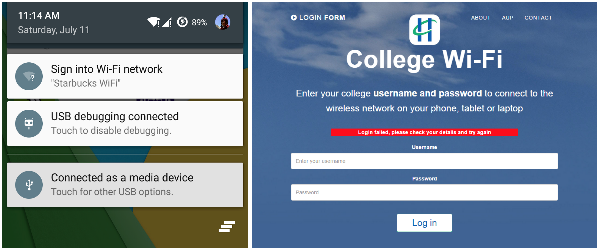
\includegraphics[width=0.75\linewidth]{./2_SensadoCol/Img/CaptivePortals.png}
\end{center}
\caption{Ejemplo de página Web que permite el acceso a Internet a través de WiFi}
\label{PortalesEjemplo}
\end{figure}
 
La solución propuesta en este TFG trataría de aunar la necesidad de monitorización de infraestructuras de la empresa y el acceso a Internet de sus usuarios, implementando un servicio de portal cautivo dotado de una aplicación web con la que se adquieren datos de los sensores del dispositivo en lugar de la clásica introducción manual de datos o credenciales a cambio de la obtención del acceso a la red.

Este sensado colaborativo podría utilizarse para diversas estadísticas (evolución temporal, mapeos de niveles...) con los que la empresa podía obtener una realimentación con unos niveles mínimos de fiabilidad. Los datos recabados no tendrían la misma calidad que el sensado realizado por equipamiento específico de alto rendimiento, pero el coste sería menor y su mantenimiento y configuración más sencillos de realizar. Además, esta solución software tendría una alta escalabilidad y versatilidad de configuraciones, por ejemplo pudiendo permitir el acceso a Internet a cambio de obtención de datos en intervalos regulares en los que el portal cautivo debe mantenerse abierto en alguna ventana o pestaña del navegador, cortándose el acceso si se cierra, o dando un tiempo de acceso fijo (\emph{lease-time}) a cambio de una lectura del micrófono durante un intervalo de tiempo limitado.

\subsection{Idea básica del sistema propuesto}

Como se ha mencionado en el apartado anterior, las soluciones de portal cautivo empleadas habitualmente requieren que el usuario del servicio introduzca manualmente ciertos datos personales o credenciales o que seleccione y visualice publicidad en procesos a menudo tediosos, repetitivos o confusos. El estilo de vida actual, en su búsqueda de la inmediatez, favorece y recompensa las soluciones en las que el usuario pierde el menor tiempo posible en el proceso de acceso al servicio.

Por ello, un servicio de portal cautivo que solo requiera del sensado del dispositivo solo precisaría de la obtención de los permisos pertinentes de acceso al \emph{hardware} ya implementados en los navegadores actuales en forma de popups sencillos con la opción de aceptar o declinar tal acceso. De esta forma e incluso aunque el servicio de portal cautivo utilizado requiera de credenciales, su obtención y el subsiguiente acceso a Internet se hace de una forma mucho más rápida para el usuario, solo teniendo que aceptar y dar permiso a la aplicación web para llevar a cabo el procedimiento automáticamente (la primera vez que la utiliza en un local determinado). En la Figura \ref{LocationMicPermissions} se muestran dos ejemplos típicos de ventanas en la que se solicita permiso al usuario para que el sistema operativo (o navegador) pueda utilizar datos de los sensores del teléfono móvil.

\begin{figure}[!t]
\begin{center}
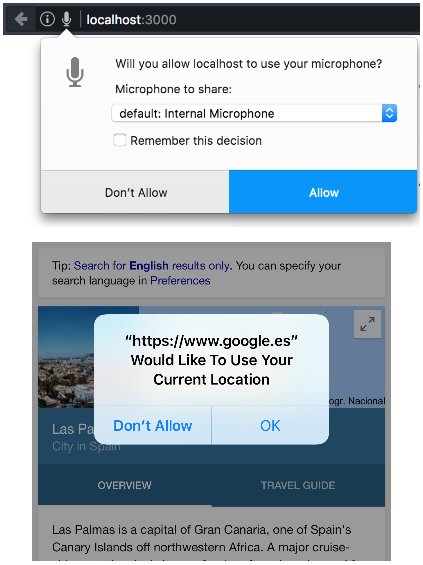
\includegraphics[width=0.5\linewidth]{./2_SensadoCol/Img/LocationMicPermissions.png}
\end{center}
\caption{Ejemplo de ventanas que solicitan permisos para usar sensores del teléfono móvil}
\label{LocationMicPermissions}
\end{figure}

Una implantación que acometa este sistema puede desarrollarse de diversas formas. En el caso de la que concierne a este TFG, se ha optado por utilizar una Raspberry Pi 3 como elemento principal del diseño (en el capítulo 4 se presenta con mayor detalle). En ella se instala todo el \emph{software} necesario para proporcionar el servicio. Se utiliza el modelo 3 de la RaspBerry Pi porque es el primero que cuenta con módulo WiFi integrado en el dispositivo, a diferencia de modelos anteriores en los que había que instalar un módulo USB aparte. En la figura \ref{SystemScheme} se muestra el esquema hardware general planteado, en el que se observa que con la interfaz WiFi de la RaspBerry Pi 3 permitimos que los usuarios se conecten al encaminador que proporciona acceso a Internet de forma controlada.

\begin{figure}[!t]
\begin{center}
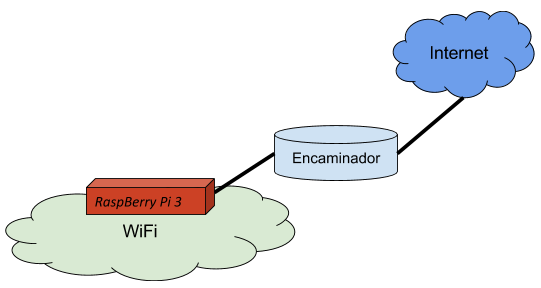
\includegraphics[width=0.75\linewidth]{./2_SensadoCol/Img/SystemScheme.png}
\end{center}
\caption{Esquema general de la infraestructura para proporcionar acceso a Internet mediante una aplicación de sensado móvil colaborativo}
\label{SystemScheme}
\end{figure}

La idea básica de la funcionalidad del sistema de sensado móvil colaborativo implantado es que aquel usuario que desee acceder a Internet, estando en la instalación de un centro que lo permita a través de su WiFi, simplemente permitiría (una sola vez) el uso del micrófono de su teléfono móvil para sensar ruido o sonido que le rodea. A cambio obtiene unos minutos de acceso gratuito a Internet. De esta forma simplificamos el proceso típico de acceder a un portal cautivo con complejos procesos de autorización (cada vez que se desea acceder a Internet). Esto supone un beneficio adicional para el usuario. Además, el propietario del local puede obtener mapas de ruido o sonido de su local a partir del sensado distribuido que hacen los distintos usuarios. Estamos pues ante un escenario en el que no todos los miembros que colaboran tienen exactamente el mismo objetivo; pero todos obtienen un beneficio en la colaboración: el usuario accede a Internet de forma gratuita, el propietario obtiene mapas de ruido con un \emph{hardware} muy barato.

Hasta donde alcanza nuestro conocimiento, no sabemos de ninguna solución similar a ésta, lo que ahonda en la novedad de este TFG. 